\documentclass{article}
\usepackage[utf8]{inputenc}
\usepackage[margin = 2cm]{geometry}
\usepackage{graphicx}
\usepackage{float}
\usepackage{caption}
\usepackage{subcaption}
\usepackage{amsmath}
%\usepackage{wrapfig}

\title{Compte Rendu - TP Musique}
\author{
CHAHRIAR Benoît}
\date{15/05/2019}

\begin{document}

\maketitle

\section{Le programme principal d'un point de vue traitement d'image}

	Ici on va voir le fonctionnement global de notre programme de la mise sous tension de la carte au traitement des images acquises par la caméra durant la partie.

	\subsection{Initialisations}

		On ouvre la capture vidéo sur un fichier vidéo ou sur une caméra selon si l'on est en train de tester en direct ou non. Ensuite on crée des trackbars qui permettent de faire des réglages manuels lors des phases de test des traitements.

	\subsection{Boucle pré-partie}

		Avant d'appliquer les traitements on attend le signal de début de partie transmis sans fil comme décrit dans la partie réseau. Durant le temps d'attente on laisse tourner le programme de de détection de la zone afain de moyenner et donc de fiabiliser les informations reçues pour le calibrage des couleurs et de la correction.

	\subsection{Boucle principale}
		On acquiert les valeurs des trackbars puis on appelle une fonction qui effectue les principaux traitements. Cette structure avait été choisie car on pensait paralléliser des traitements de frame-une image extraite du flux vidéo- nous même pour améliorer la vitesse de traitement. On a ensuite réaliser en testant le programme qu'open cv était multi threadé de base.
		En utilisant la zone détéctée automatiquement on corrige la perspective de l'image. Ensuite on passe la l'image capturée du domaine BGR au domaine HSV, car il est bien plus simple d'isoler une couleur en HSV. Le caractère coloré d'un pixel est seuillé par la saturation et la , et un simple passe bande dans les teintes - Hue - isole facilement la couleur voulue. On floute l'image - effet passe-bas - puis si on est en mode automatique on utilise la matrice stockant les couleurs donnée à l'initialisation pour appliquer un passe bande autour de ce seuil, un par couleur. On trace ensuite tous les contours sur chacune des trois images seuillées : rouge, vert et bleue. On procède à une ouverture pour éliminer les petites zones détéctées à tord. On calcule ensuite la position des centres des contours et enfin on trie ces centres. La zone cible des palets est très colorée et mène à de nombreux faux positifs donc on élimine les centres détéctés dans cette portion de l'image. On élimine aussi le bord inférieur de l'image car la partie en bois du support de terrain entre dans le champ et est aussi détectée. Les coordonnées sont ensuite prêtes à être transmises par wifi.

\section{Explications supplémentaires}

\subsection{Trouver le centre à partir d'un contour}
	Pour trouver la position du centre à partir des contours identifiés on fait appel au moment d'ordre 0 et 1.

	\begin{equation*}
		m_ij = \sum_{xy}^{} x*y*x^{i}*x^{j}
	\end{equation*}
	\begin{equation*}
		x = \frac{m_{10}}{m_{00}}
	\end{equation*}
	\begin{equation*}
		y = \frac{m_{01}}{m_{00}}
	\end{equation*}
	Note : En arrière plan, Opencv utilise le théorème de Green qui fait le lien entre le contour et la surface entourée par le contour simple - sans boucles -.


\subsection{L'ouverture d'une image}
	L'ouverture est une opération composée de deux opérations élémentaires de morphologie mathématique. Le principe est d'utiliser un élément structurant pour traiter notre image selon certaine règle.
	Pour l'érosion on considère un pixel ou l'on place notre élément structurant. Le pixel considéré prendra la valeur minimale présente dans son voisinage défini par l'élément structurant.
	La dilatation est la même opération mais on garde la valeur maximale.
	L'ouverture pour effect de supprimer les petits éléments isolés dont la dimension est inférieure à l'élément structurant de notre image binaire tout en assurant de ne pas trop altérer la taille des palets en redilatant par la suite.
	% \begin{figure}[H]
	% \centering
 %      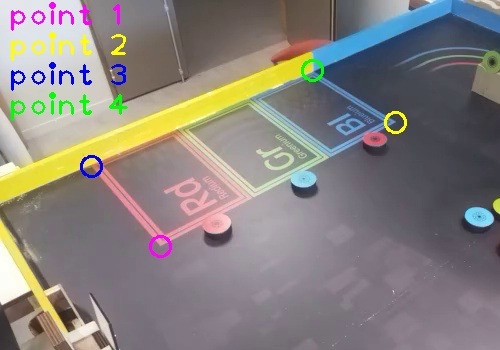
\includegraphics[height=4cm]{image_4_points.jpg}
	% \end{figure} 




\end{document}
